\documentclass[12pt]{article}

%Packages Used%
\usepackage{amsmath}
\usepackage{amssymb}
\usepackage{latexsym}
\usepackage{amsfonts}
\usepackage{graphicx}
\graphicspath{ {images/} }



\usepackage[margin=1in]{geometry}


\setlength{\abovedisplayskip}{3mm}
\setlength{\belowdisplayskip}{3mm}
\setlength{\abovedisplayshortskip}{0mm}
\setlength{\belowdisplayshortskip}{2mm}
\setlength{\baselineskip}{12pt}
\setlength{\normalbaselineskip}{12pt}

\newcommand{\blank}{\underline{~~~~~~~~~}}
\newcommand{\RR}{\mathbb{R}}
\newcommand{\CC}{\mathbb{C}}
\newcommand{\ZZ}{\mathbb{Z}}
\newcommand{\PP}{\mathbb{P}}
\newcommand{\FF}{\mathbb{F}}
\newcommand{\kk}{\mathbf{k}}
\newcommand{\cP}{\mathcal{P}}

\newcommand{\bu}{\mathbf{u}}
\newcommand{\bv}{\mathbf{v}}
\newcommand{\bx}{\mathbf{x}}
\newcommand{\by}{\mathbf{y}}
\newcommand{\bb}{\mathbf{b}}
\newcommand{\bc}{\mathbf{c}}
\newcommand{\bp}{\mathbf{p}}
\newcommand{\bq}{\mathbf{q}}
\newcommand{\be}{\mathbf{e}}
\newcommand{\bzero}{\mathbf{0}}
\DeclareMathOperator{\Nul}{Nul}
\DeclareMathOperator{\Mod}{mod}
\DeclareMathOperator{\ord}{ord}
\DeclareMathOperator{\GL}{GL}
\DeclareMathOperator{\SL}{SL}
\DeclareMathOperator{\Hom}{Hom}
\DeclareMathOperator{\End}{End}
\DeclareMathOperator{\Ind}{Ind}
\DeclareMathOperator{\im}{im}
\DeclareMathOperator{\tr}{tr}

\renewcommand{\And}{\wedge}
\newcommand{\Or}{\vee}



\normalbaselines
\pagestyle{empty}
\raggedbottom
\begin{document}

%\begin{comment}
\textbf{Name:} Yihan Zhou \smallskip  
\textbf{GT account:} yzhou376@gatech.edu\smallskip \\ 
\textbf{GT number:} 903053761\smallskip \\ 

\begin{center}
{
CS 4641  Machine Learning \\
HW2 \\

}

\end{center}

Problems Set

\begin{itemize}



\item[1.] \smallskip To set $\alpha_k$ to be constant means the learning rate will not change throughout the whole learning process. While to set $\alpha_k$ as function $k$ means the learning rate is adaptable to learning time.

\end{itemize}

\begin{itemize}

\item[2.a. ] \smallskip Because $\textbf{w}$ is perpendicular to the decision boundary, it should be parallel to \\  $\phi(x_2) - \phi(x_1)$. which is $
\left[\begin{array}{c} 
1 \\ \sqrt{2} \cdot \sqrt{2} \\ \sqrt{2}^2
\end{array}\right] - 
\left[\begin{array}{c} 
1 \\ \sqrt{2}\cdot0 \\ 0^2
\end{array}\right] 
= 
\left[\begin{array}{c} 
0 \\ 2 \\ 2
\end{array}\right] $  

\end{itemize}

\begin{itemize}

\item[2.b. ] \smallskip Margin is the Euclidean distance between the two points. We get $\sqrt{0^2 + 2^2 + 2^2} = 2\sqrt{2}$.

\end{itemize}



\begin{itemize}

\item[2.c. ] \smallskip According to definition, $  \sqrt{2} = \frac{2}{\|\textbf{w}\|_{2}}$. Thus we solve $\|\textbf{w}\|_{2} = \dfrac{1}{\sqrt{2}}$. Since $\textbf{w}$ is parallel to $\left[\begin{array}{c} 
0 \\ 2 \\ 2
\end{array}\right]$, we get $\textbf{w} = \left[\begin{array}{c} 
0 \\ 0.5 \\ 0.5
\end{array}\right]$.


\end{itemize}

\begin{itemize}

\item[2.d. ] \smallskip We substitute the value of $\textbf{w}, y_1$, and $y_2$ back into the inequality and get $$ -1 \cdot ( \left[\begin{array}{c} 
0 \\ 0.5 \\ 0.5
\end{array}\right] 
\left[\begin{array}{c} 
1 \\ \sqrt{2}\cdot0 \\ 0^2
\end{array}\right]+w_0) \geq 1$$
$$ 1 \cdot ( \left[\begin{array}{c} 
0 \\ 0.5 \\ 0.5
\end{array}\right] 
\left[\begin{array}{c} 
1 \\ \sqrt{2} \cdot \sqrt{2} \\ \sqrt{2}^2
\end{array}\right]+w_0) \geq 1$$
By calculation, we get $$ -w_0 \geq 1$$ $$2+w_0\geq1$$ $$w_0\leq-1$$ Thus, $$w_0=-1$$.

\end{itemize}

\begin{itemize}

\item[2.e. ] \smallskip We substitute all the elements back and get $$h(x) = -1 + \frac{\sqrt{2}}{x}x + \frac{1}{2}x^2$$



\end{itemize}

Implementation Short Answers


\begin{itemize}

\item[2.3. ] \smallskip As we increase the lambda, we ‘blur’ the boundary, which leads probability to be less deterministic. As we decrease the lambda, the result turned to be more polarized. As we increase the lambda, bias increase and variance decrease. As we decrease the lambda, bias decrease and variance increase. (Plots are attached at the end of the pdf. Please check them there. Thx!! )


\begin{figure}[h]
\caption{Lambda=0.0000001(Probability)}
\centering
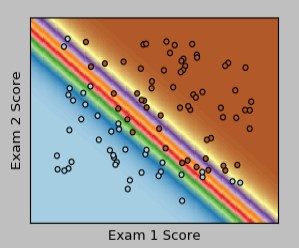
\includegraphics[width=0.5\textwidth]{l01p}

\caption{Lambda=0.0000001(Threshold)}
\centering
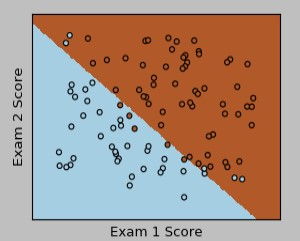
\includegraphics[width=0.5\textwidth]{l01t}

\caption{Lambda=10(Probability)}
\centering
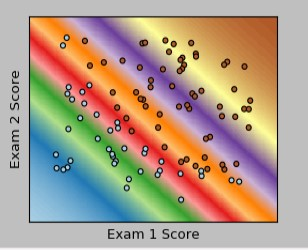
\includegraphics[width=0.5\textwidth]{l10p}
\end{figure}

\begin{figure}[h!]
\caption{Lambda=10(Threshold)}
\centering
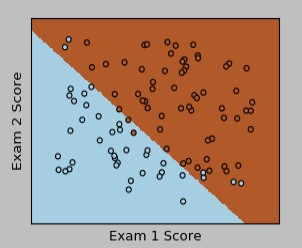
\includegraphics[width=0.5\textwidth]{l10t}

\caption{Lambda=100(Probability)}
\centering
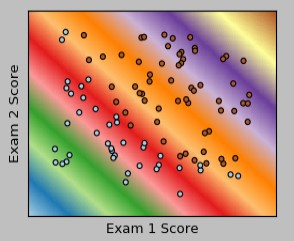
\includegraphics[width=0.5\textwidth]{l100p}

\caption{Lambda=100(Threshold)}
\centering
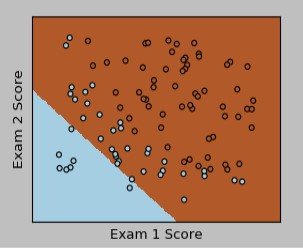
\includegraphics[width=0.5\textwidth]{l100t}
\end{figure}


\end{itemize}

\begin{itemize}

\item[3.4. ] \smallskip 
Poly: As we increase the degree in SVM polynomial Kernel, the decision boundary tends to be increasingly complicate curve. Biases decreases while variances increases,  which cause over-fitting on training data. As we increase the C in SVM, the decision boundary also increasingly classifies all training data correct, but tends to lose natural separation between the data.Biases decreases while variances increases,  which also cause over-fitting on training data.\\
Gaussian: 
As we decrease the sigma in SVM Gaussian Kernel, the decision boundary tends to be increasingly fits every data, and finally converge around some data point. Biases decreases while variances increases,  which cause over-fitting on training data.  As we increase the C in SVM, the decision boundary also increasingly classifies all training data correct, decreases biases while increases variances,causing over-fitting on training data.\\    



\end{itemize}


\end{document}
